\chapter{Frequency Domain Analysis}
\label{chap:frequency-domain}

%%%%%%%%%%%%%%%%%%%%%%%%%%%%%%%%%%%%%%%%%%%%%%%%%%%%%%%%%%%%
\section{Linear Time-Invariant Systems}
\label{sec:LTI}

We consider linear time-invariant systems
\begin{equation}
  \label{eq:linear-model-pulse}
  y(k) \doteq \sum_{l=1}^\infty g(l)u(k-l) + v(k)
\end{equation}
with a causal pulse reponse $g(l)=0$, $\forall l\le 0$.

Using the \emph{forward and inverse shift operator}~\cite[p.~24]{ljung}
\begin{equation*}
  qu(k) \doteq u(k+1), \hspace{2em} q^{-1}u(k) \doteq u(k-1)
\end{equation*}
one rewrites the expression above as
\begin{equation*}
  \sum_{l=1}^\infty g(l)u(k-l) = \sum_{l=1}^\infty g(l)q^{-l}u(k) = \underbrace{\left[\sum_{l=1}^\infty g(l)q^{-l}\right]}_{\doteq G(q)}u(k).
\end{equation*}

$v(t)$ is a filtered additive disturbance, $v(t)=H(q)e(t)$
\begin{equation*}
  H(q) \doteq 1 + \sum_{l=1}^\infty h(l)q^{-l}
\end{equation*}
and $e(k)$ is scaled so that $h(0)=1$.

In the rest, we shall be considering the (SISO) linear model
\begin{equation}
  \label{eq:linear-model-z}
  y(k) = G(z)u(k) + H(z)e(k)
\end{equation}
where $y,u \in \mathcal{R}$, $e \in \mathcal{N}(0,\sigma^2)$ is the Gaussian uncorrelated independent and identically distributed (i.i.d.) noise with zero mean and variance $\sigma^2$ and $v(k) = H(z)e(k)$ the filtered noise.

We wish to estimate $\hat{G}$ from the finite set of measurements
\begin{equation*}
  \mathcal{Z}_K = \{u(0),y(0),\ldots,u(K-1),y(K-1))\}
\end{equation*}
of length $K$. The different methods
\begin{itemize}
\item transfer function in the frequency domain (this Chapter);
\item real-rational transfer function in the time domain\footnote{
    This holds for the frequency and the time approach. Eq.~\eqref{eq:linear-model-z} is parametrized as
    \begin{equation*}
      y(k) = G(\theta)u(k) + H(\theta)e(k),\hspace{1em}y \in \mathcal{R},\ u\in \mathcal{R}
    \end{equation*}
    where $\theta \in \mathcal{R}^d$ and $d$ is the model parameter. For real-rational transfer functions in the $z$-domain
    \begin{equation}
      %\label{eq:transfer-function-parametrization}
      G(z) = \frac{b_1z^{-1} + b_2z^{-2} + \ldots + b_mz^{-m}}{1 + a_1z^{-1} + \ldots + a_mz^{-n}}
    \end{equation}
    a common parametrization is
    \begin{equation*}
      \theta =
      \begin{bmatrix}
        a_1 & \ldots & a_n & b_1 & \ldots & b_m
      \end{bmatrix}^\top
    \end{equation*}
    where $p = m+n$. The transfer function in the frequency domain $G(\ejw)$ is $G(z)$ evaluated at fixed points $z=\ejw$
    \begin{equation*}
      G(\ejw) = G(z)\Big|_{z=\ejw}.
    \end{equation*}}, Chap.~\ref{chap:time-domain};
\item state-space approach
  \begin{equation*}
    \begin{aligned}
      x(k+1) &= Ax(k) + Bu(k) \\
      y(k) &= Cx(k) + Du(k)
    \end{aligned}
  \end{equation*}
  Chap.~\ref{chap:state-space}.
\end{itemize}
are equivalent in the absence of noise. For all methods, the \emph{unmeasured} past induces an error in the estimate because for a causal system, the signal $y(k)$ depends on the control inputs at previous times up to time $k$ which may all not be available. The problem does not arise when the system starts at rest where $u(k)=y(k)=0,\ \forall k<0$.

%%%%%%%%%%%%%%%%%%%%%%%%%%%%%%%%%%%%%%%%%%%%%%%%%%%%%%%%%%%%
\section{Empirical Transfer-Function Estimate (ETFE)}
\label{sec:ETFE}

In the frequency domain,
\begin{equation*}
  U(\ejw) \doteq \sum_{k=-\infty}^{\infty} y(k)e^{j\omega k} \hspace{2em} Y(\ejw) \doteq \sum_{k=-\infty}^{\infty} y(k)e^{j\omega k}
\end{equation*}
eq.~\eqref{eq:linear-model-z} becomes
\begin{equation}
  \label{eq:model-frequency-domain}
  Y(\ejw) = G(\ejw)U(\ejw) + V(\ejw) + R(\ejw)
\end{equation}
where the system's response $Y(\ejw)$ has been split\footnote{The initial transient corrupts the measurements: let $W_{[0,N-1]}(k)$
  \begin{equation*}
    W_{[0,N-1]}(k) =
    \begin{cases}
      1 & \text{ if } 0\le k < N \\
      0 & \text{ otherwise}
    \end{cases}
  \end{equation*}
  the window function; then, for all times up to $N-1$,
  \begin{align*}
    y(k) &= Gu_p(k) - \underbrace{Gu_p(k)W_{(-\infty,-1]}(k)}_{r(r)} + v(k) \\
    Y_N(\ejwn) &= G(\ejwn)U_N(\ejwn) + R_N(\ejwn) + V(\ejwn)
  \end{align*}
  where $u_p(k)$ is the periodic input signal.} into a periodic term driven by the periodic input $U(\ejw)$ and the additional term $R(\ejw)$ which accounts for the transient.

To obtain an estimate $\hat{G}(\ejw)$ for $G(\ejw)$, we make the following three considerations:
\begin{itemize}
\item the ratio
  \begin{equation}
    \label{eq:EFTE}
    \frac{Y(\ejw)}{U(\ejw)}
  \end{equation}
  provides an \emph{unbiased} estimate of $G(\ejwn)$ for a periodic input signal (\textit{i.e.} no transient) and in the absence of noise (see Sect.~\ref{sec:ETFE-statistical-properties});
\item we only have access to finite length input-output data $\{u(k),y(k)\}$. As the best approximation for the infinite summation $\{U(\ejw), Y(\ejw)\}$ we use the discrete Fourier transforms (Sect.~\ref{sec:DFT})
  \begin{equation*}
    U_N(\ejwn) = \sum_{k=0}^{N-1} y(k)\ejwn[k] \hspace{2em} Y_N(\ejwn) = \sum_{k=0}^{N-1} y(k)\ejwn[k].
  \end{equation*}
  $\omega_n=\frac{2\pi}{N}$ are determined by the number of measurement points $N$;
\item the Fourier transform of $v(k)$ is assumed to exist. As noise is typically finite power, and not finite energy, this will not be satisfied. However we are more interested in the relationship between $U(\ejwn)$ and $Y(\ejwn)$ and so we will overlook this issue for the time being.
\end{itemize}

%%%%%%%%%%%%%%%%%%%%%%%%%%%%%%%%%%%%%%%%%%%%%%%%%%%%%%%%%%%%
\subsection{Effect of the Input Signal}
\label{sec:ETFE-statistical-properties}

The statistical properties of the EFTE
\begin{equation}
  \label{eq:freq-domain-LTI-estimator}
  \hat{G}(\ejwn) \doteq \frac{Y_N(\ejwn)}{U_N(\ejwn)} = G(\ejwn) + \frac{R_N(\ejwn)}{U_N(\ejwn)} + \frac{V_N(\ejwn)}{U_N(\ejwn)}
\end{equation}
are affected by how the input signal is chosen. The estimate is unbiased, since $\EE{V_N(\ejwn)}=0$,
\begin{equation*}
  \EE{\hat{G}(\ejwn)} = G(\ejwn) + \frac{R_N(\ejwn)}{U_N(\ejwn)}
\end{equation*}
and in the absence of the transient, $R_N(\ejwn)=0$, that is, for a \emph{periodic} signal\footnote{Periodicity implies that the input signal is known in the interval $[-\infty,+\infty]$ and that the transient has already died out. This is not the case for a random input signal even if the input starts at times earlier than $k=0$ unless the initial conditions are known: in this case the transient could be taken into account, see Sect~\ref{chap:time-domain}}.

The choice of input signal also affects the signal-to-noise ratio (SNR): if the number of measurement points $N$ is taken to be a multiple integer of the period $M$ of the input signal, the magnitude of $U_N(e^{j\omega})$ grows at a rate of $N$
\begin{equation}
  \label{eq:PSD-periodic-input-signal}
  \EE{\left|U_N(\ejwn)\right|^2} = m^2\left|U_M(\ejwn)\right|^2,\hspace{2em} m=\frac{N}{M}.
\end{equation}
Here the only frequencies with non-zero spectral amplitude are those at $\frac{2\pi}{M}n$ with $n\in [0,\ldots,M-1]$, since the signal is periodic with period $M$, even though there are $N$ measurement points; the remaining $N-M$ components are 0.

Were instead the input signal \emph{random}, we would have
\begin{equation}
  \label{eq:PSD-random-input-signal}
  \EE{|U_N(\ejwn)|^2} = N\phi_u(\ejwn) + 2c
\end{equation}
where here \emph{all} $N$ frequencies $\frac{2\pi}{N}n$ have spectral content. In other words, a periodic signal excites only a limited number of frequencies and concentrates all the energy in those frequencies, a random one the whole spectrum. The quantity
\begin{equation*}
  |c| \le C = \sum_{\tau=1}^\infty |\tau R_v(\tau)|
\end{equation*}
is finite for random noise (50~Hz noise is not finite).

\begin{figure}[h]
  \centering
  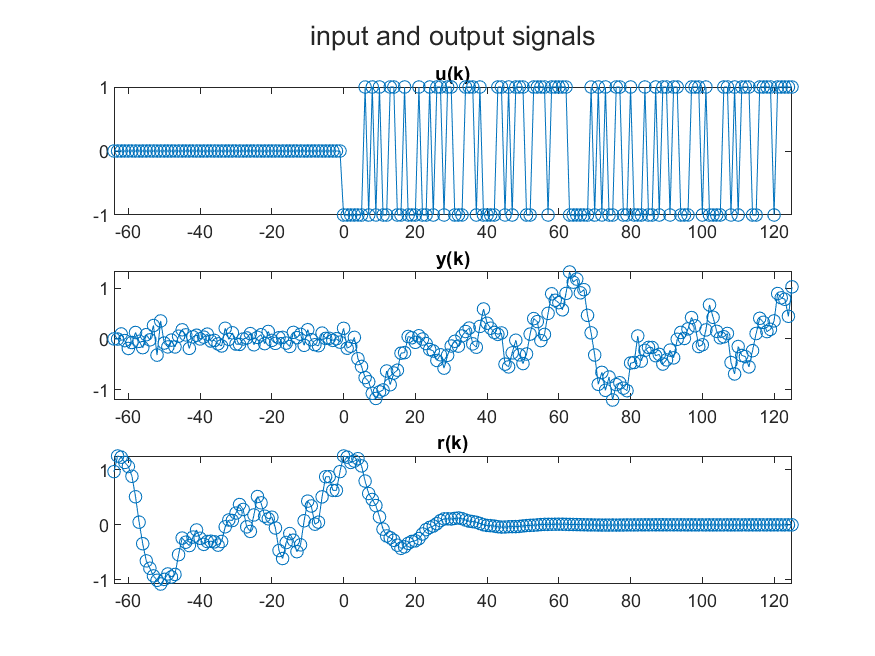
\includegraphics[width=0.8\textwidth]{"05_lect/transient-noise-time-domain.png"}
  \caption{Plot of the input $u(k)$ (top), the output $y(k)$ (middle) and transient $r(k)$ (bottom) signals, here shown only for two periods before $t=0$ and two after $t=0$.}
  \label{fig:transient-response-time-domain}
\end{figure}

What is the impact of the noise\footnote{For a periodic input signal, we have
  \begin{equation}
    \label{eq:variance-ETFE}
    \mathbb{E}\left\{\left|\hat{G}_N(e^{j\omega_n}) - G_0(e^{j\omega_n})\right|^2\right\} = \frac{\phi_v(e^{j\omega_n}) + \frac{2c}{N}}{\frac{1}{N}|U_N(e^{j\omega_n})|^2}
  \end{equation}
  the expression for $c$ is given above, and
  \begin{equation*}
    \EE{|\hat{G}(\ejwn)|^2} = |G(\ejwn)|^2 + \frac{N\phi_v(\ejwn)}{|U_N(\ejwn)|^2}.
  \end{equation*}} and the transient? What follows is my hand-waving attempt to understand the motivation to use a periodic signal. The noise signal ``behaves'' like a random input signal: disregarding the constant term in eq.~\eqref{eq:PSD-random-input-signal}, SNR remains constant for a random input signal, since
\begin{equation*}
  \frac{\EE{|V_N(\ejwn)|^2}}{\EE{|U_N(\ejwn)|^2}}
\end{equation*}
does not change for growing $N$. Instead it decreases as $\frac{1}{N}$ for periodic input signals.

\begin{figure}[h]
  \centering
  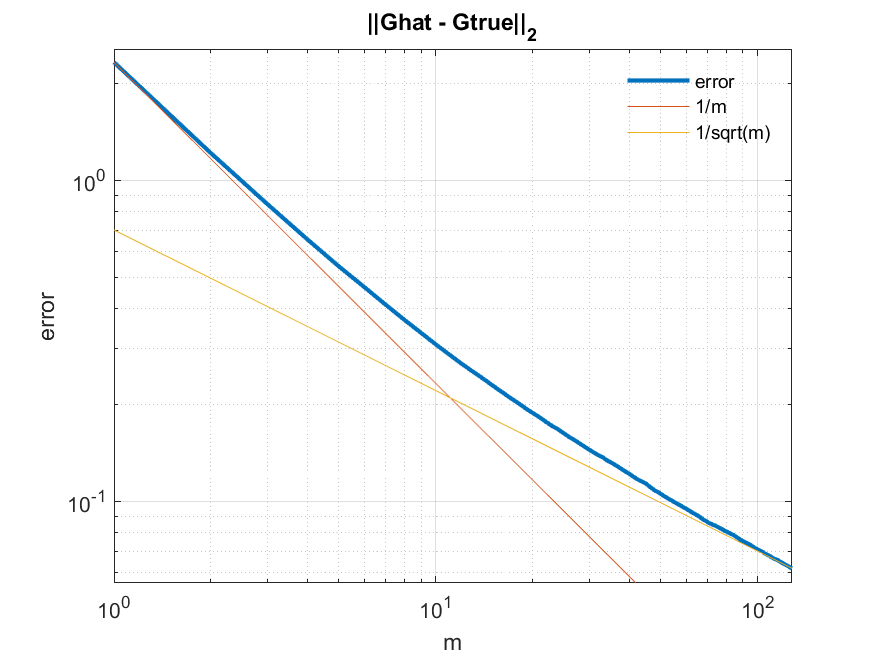
\includegraphics[width=0.8\textwidth]{"05_lect/transient-noise-convergence-avg.png"}
  \caption{Convergence of $\EE{||\hat{G}-G||_2}$ as a function of the number of periods $m$ (each of M points). The cross-over between the transient-limited convergence with dependence $\frac{1}{m}$ to noise-limited with convergence $\frac{1}{\sqrt{m}}$ is clearly visible.}
  \label{fig:transient-response-convergence}
\end{figure}

The transient instead decays exponentially: its PSD remains constant as a function of $N$ and the convergence of the SNR is $\sim\frac{1}{N}$. Fig.~\ref{fig:transient-response-time-domain} shows the output signal $y(k)$ affected by both noise and transient: the cross-over between transient-limited and noise-limited convergence is visible in Fig.~\ref{fig:transient-response-convergence}. Implementation in \texttt{05\_lect/SysID\_ETFE.m}.


%%%%%%%%%%%%%%%%%%%%%%%%%%%%%%%%%%%%%%%%%%%%%%%%%%%%%%%%%%%%
\section{Swept-Sine Identification}
\label{sec:swept-sine-identification}

The system\footnote{To my knowledge, this method is also called demodulation or lock-in detection.} is excited with the periodic input signal $u(k)=\alpha \cos(\omega_uk)$ of \emph{arbitrary} frequency $\omega_u$. The output\footnote{Plugging the excitation into eq.~\eqref{eq:linear-model-pulse}, one obtains
  \begin{align*}
    y(k) &= \frac{\alpha}{2}\left[\sum_{l=1}^\infty g(l) e^{+j\omega_u(k-l)} + \sum_{l=1}^\infty g(l) e^{-j\omega_u(k-l)}\right] + v(k) \\
         &= \frac{\alpha}{2}\left[\left(\sum_{l=1}^\infty g(l) e^{-j\omega_ul}\right) e^{+j\omega_uk} + \left(\sum_{l=1}^\infty g(l) e^{+j\omega_ul}\right) e^{-j\omega_uk}\right] + v(k)
  \end{align*}
  where the terms in round brackets are $G(e^{+j\omega_u})$ and $G(e^{-j\omega_u})$ respectively.} to this excitation is
\begin{equation*}
  y(k) = \underbrace{\frac{\alpha}{2} \left[G(e^{j\omega_u})e^{+j\omega_uk} + G(e^{-j\omega_u})e^{-j\omega_uk}\right]}_\text{steady state response} + v(k) + \text{transient}.
\end{equation*}
The correlation signal
\begin{align*}
  I(N) &\doteq \frac{1}{N}\sum_{k=0}^{N-1}y(k)e^{-j\omega_u k} \\
       &= \frac{\alpha}{2} G(e^{j\omega_u}) + \frac{\alpha}{2N} \sum_{k=0}^{N-1} G(e^{j\omega_u})e^{-2j\omega_u k} \\
       &\rightarrow \frac{\alpha}{2} G(e^{j\omega_u})\hspace{1em} \text{as } N\rightarrow \infty
\end{align*}
since the non-contant components (including noise and transient) average out.

Advantages of this method:
\begin{itemize}
  \itemsep0em
\item the energy is concentrated at the frequencies of interest;
\item arbitrary frequencies can be measured and not only those determined by the Fourier transform;
\item the amplitude of $u(k)$ can easily be tuned as a function of frequency;
\item it makes it easy to avoid saturation and to tune SNR.
\end{itemize}
Disadvantages are:
\begin{itemize}
  \itemsep0em
\item a large amount of data is required;
\item significant amount of time required for experiments because single frequencies are probed sequentially;
\item some processes will not allow sinusoidal inputs.
\end{itemize}


%%%%%%%%%%%%%%%%%%%%%%%%%%%%%%%%%%%%%%%%%%%%%%%%%%%%%%%%%%%%
\section{Spectral Estimation Methods}
\label{sec:spectral-estimation-methods}

From eq.~\eqref{eq:freq-domain-LTI-estimator}, neglecting the transient and multiplying element-wise\footnote{The supplementary notes take a different approach, so I am not sure that my derivation holds.} by $U^\star(\ejwn)$, we have
\begin{equation*}
  \phi_{yu}(\ejwn) = G(\ejwn) \phi_u(\ejwn) + \phi_{uv}(\ejwn)
\end{equation*}
the cross correlation term $\phi_{uv}(\ejwn)$ being zero if $u$ and $v$ are uncorrelated (for instance in open loop). The estimate $\hat{G}(\ejwn)$ is
\begin{equation*}
  \hat{G}(\ejwn) = \frac{\hat{\phi}_{yu}(\ejwn)}{\hat{\phi}_u(\ejwn)}.
\end{equation*}

It is not clear to me why one would choose spectral methods instead of ETFE since the difference is only the multiplication by the deterministic input signal.

The major point is how to determine the PSD in the case of non-periodic signals.

\iffalse
  %%%%%%%%%%%%%%%%%%%%%%%%%%%%%%%%%%%%%%%%%%%%%%%%%%%%%%%%%%%%
  \section{Smoothed Correlation and Cross-Correlation}
  \label{sec:smoothed-correlations}

  The estimate $\hat{G}(e^{j\omega})$ can be smoothed using a window function $W(e^{j\omega})$:
  \begin{equation*}
    \tilde{G}_N(e^{j\omega}) = \sum_{\xi=-\frac{N}{2}+1}^{\frac{N}{2}} W_\gamma(e^{j(\xi-\omega_n)}) \alpha(e^{j\xi}) \hat{G}_N(e^{j\xi})
  \end{equation*}
  where $\alpha$ is the variance weighting of the result. The calculation is however better performed as multiplications after Fourier transformation.

  % What is the value to use for the variance?

  Filtering is usually done by the Hann function or by raised cosine. Its Fourier transform is real because the function is symmetric with respect to $k$\footnote{One has
    \begin{equation*}
      X(\ejwn) = \sum_{k=0}^{N-1} x(k)[\cos(\omega_nk) - j\sin(\omega_nk)].
    \end{equation*}
  }.
\fi

%%%%%%%%%%%%%%%%%%%%%%%%%%%%%%%%%%%%%%%%%%%%%%%%%%%%%%%%%%%%
\section{Discrete Fourier Transform}
\label{sec:DFT}

The Fourier series is defined (for $M$ even) as
\begin{equation}
  \label{eq:fourier-transform}
  X(\ejwn) = \sum_{k=0}^{M-1} x(k) \emjwn[k],\hspace{2em} \omega_n = \frac{2\pi}{M}n
\end{equation}
and the inverse Fourier transform as
\begin{equation}
  \label{eq:inverse-fourier-transform}
  x(k) = \frac{1}{M}\sum_{n=0}^{M-1} X(\ejwn) \ejwn[k].
\end{equation}

%%%%%%%%%%%%%%%%%%%%%%%%%%%%%%%%%%%%%%%%%%%%%%%%%%%%%%%%%%%%
\subsection{Auto-Correlation for Periodic Signals}
\label{sec:autocorrelation-periodic}

Given the periodic signal $\{x(k)\}$, the auto-correlation function is the product of $x$ with itself delayed by $\tau$:
\begin{equation}
  \label{eq:auto-correlation}
  R_x(\tau) = \frac{1}{N}\sum_{k=0}^{N-1} x(k)x(k-\tau)
\end{equation}
and the power spectral density (PSD)\footnote{Using $\emjwn[\tau] = \emjwn[k]\cdot \emjwn[(\tau-k)]$ and eq.~\eqref{eq:auto-correlation}, one has
  \begin{align*}
    \phi_x(\ejwn) &= \frac{1}{N}\sum_{k=0}^{N-1} x(k)e^{\emjwn[k]} \left[\sum_{\tau=0}^{N-1} x(k-\tau)\emjwn[(k-\tau])\right]^\star \\
                  &= \frac{1}{N}X(\ejwn) X^\star(\ejwn)
  \end{align*}
}
\begin{equation}
  \label{eq:PSD}
  \phi_x(e^{j\omega_n}) = \sum_{\tau=0}^{N-1} R_x(\tau) e^{-i\omega_n\tau} = \frac{1}{N}|X(e^{j\omega_n})|^2.
\end{equation}

The auto-correlation has the following properties:
\begin{itemize}
\item $R_x(-\tau) = R_x^\star(\tau)$;
\item $R_x(0)\ge |R_x(\tau)|$, for all $\tau>0$.
\end{itemize}
$\phi_x(\omega)$ has the following properties:
\begin{itemize}
\item $\phi_x(\omega)$ is non-negative for all $\omega$
\item $\phi_x(\omega) = \phi_x(-\omega)$ for all real-valued $x(k)$.
\end{itemize}

%%%%%%%%%%%%%%%%%%%%%%%%%%%%%%%%%%%%%%%%%%%%%%%%%%%%%%%%%%%%
\subsection{Cross-Correlation for Periodic Signals}
\label{sec:crosscorrelation-periodic-signals}

Given the periodic signals $y(k)$ and $u(k)$, the cross-correlation function is
\begin{equation}
  \label{eq:cross-correlation}
  R_{yu}(\tau) = \frac{1}{N}\sum_{k=0}^{N-1} y(k)u(k-\tau)
\end{equation}
and the cross-spectral density
\begin{equation}
  \label{eq:cross-correlation-PSD}
  \phi_{yu}(\ejwn) = \sum_{\tau=0}^{N-1} R_{yu}(\tau) e^{-i\omega_n\tau} = \frac{1}{N}Y(\ejwn)U^\star(\ejwn).
\end{equation}


%%%%%%%%%%%%%%%%%%%%%%%%%%%%%%%%%%%%%%%%%%%%%%%%%%%%%%%%%%%%
\section{Random Signals}
\label{sec:random-signals}

We assume $e(k)\in \mathcal{N}(0,\sigma^2)$; $e(k)$ are independent and identically distributed (i.i.d.).

For random signals, the definition is in terms of the expected values: the \emph{autocorrelation} function is defined as
\begin{equation*}
  R_x(\tau) = \EE{x(k)x(k-\tau)}
\end{equation*}
and the \emph{covariance} function as
\begin{equation*}
  R_x(\tau) = \EE{\left(x(k) - \EE{x}\right)\left(x(k-\tau)-\EE{x}\right)}
\end{equation*}
It will be assumed that random signals are zero mean and the notation $R_x(\tau)$ is used for both the autocorrelation and covariance functions. The stationarity implies that the expectations only depends on the shift $\tau$.

The power spectral density is defined as the \emph{Fourier transform} of the autocovariance, $R_x(\tau)$
\begin{equation*}
  \phi_x(\ejw) = \sum_{\tau=-\infty}^\infty R_x(\tau)e^{-j\omega\tau} \hspace{1em} \omega\in[-\pi,\pi)
\end{equation*}
and the inverse transform is given by
\begin{equation*}
  R_x(\tau) = \frac{1}{2\pi}\int_{-\pi}^{+\pi} \phi_x(e^{j\omega})e^{j\omega\tau}\du \omega.
\end{equation*}

Cross-covariance and cross-correlations are similarly defined. For zero mean signals, the cross-correlation is
\begin{equation*}
  R_{yu}(\tau) = \EE{y(k)u(k-\tau)}.
\end{equation*}

The definitions for the auto- and cross-correlation given above are for infinite length signals. Since one can only collect finite-length data, one must make a sensible approximation. The difficulty arises from the fact that in system identification ``the measured output is almost always composed of the sum of a stochastic signal (from the noise) and a deterministic, or even periodic, signal from the convolution of the plant with a deterministic input signal, $u(k)$. This means that there is no obvious correct choice in deciding which autocorrelation estimation method to apply. The better method will inevitably be problem dependent.''~\cite{smith-suppl4}.

\iffalse
  %%%%%%%%%%%%%%%%%%%%%%%%%%%%%%%%%%%%%%%%%%%%%%%%%%%%%%%%%%%%
  \section{Periodogram}
  \label{sec:periodogram}

  If $\{s(t)\}$ and $\{w(t)\}$ are related by the strictly stable system $G(q)$ and the input for $t<0$ unknown but obeying $|w(t)|\le C_w$ for all $t$, one has
  \begin{equation}
    \label{eq:filtered-periodogram-estimate}
    S_N(w) = G(e^{i\omega})W_N(w) + R_N(w)
  \end{equation}
  where
  \begin{equation}
    \label{eq:estimate-transient}
    |R_N(w)| \le 2C_w\frac{C_G}{\sqrt{N}},\hspace{2em} C_G = \sum_{k=1}^\infty k|g(k)|
  \end{equation}
  $R_N$ is \emph{not} the transient response.

  This is defined for or a random signal

  \begin{equation*}
    \frac{1}{N}\left|V_N(\ejw)\right|^2
  \end{equation*}
  is an asymptotically unbiased estimator of the spectrum
  \begin{equation*}
    \lim_{N\rightarrow \infty} \EE{\frac{1}{N} \left|V_N(\ejw)\right|^2} = \phi_v(\omega)
  \end{equation*}
  under the assumption that the autocorrelation decays quickly enough
  \begin{equation*}
    \lim_{N\rightarrow \infty} \frac{1}{N} \sum_{\tau=-N}^N |\tau R_v(\tau)| = 0
  \end{equation*}
\fi

%%% Local Variables:
%%% mode: latex
%%% TeX-master: "notes"
%%% End:
